\section{The Pulsar/\Actitle{PWN} System}
\seclabel{pulsar_pwn_system}

\subsection{Neutron Star Formation}

As was discussed in \secref{astrophysical_sources}, pulsars, 
\acp{PWN},
and supernova remnants are all the end products of supernovas.  When a
star undergoes a supernova, the ejecta forms a supernova rememant.  If the
remaining stellar core has a mass above the Chandrasekhar limit,
then the core's electron degeneracy pressure cannot counteract the core's
gravitational force and the core will collapse into a neutron star.
The Chandrasekhar mass limit can be
approximated as \citep{chandrasekhar_1931_maximum-ideal}
\begin{equation}
  \MassChandrasekhar \approx 
  \frac{3\sqrt{2\pi}}{8}
  \left(\frac{\hbar\speedoflight}{\gravitationalconstant}\right)^{3/2}
  \left[
  \left(\frac{\NumberProtons}{\NumberNucleons}\right)
  \frac{1}{\MassHydrogen^2}
  \right]
\end{equation}
where $\hbar$ is the reduced Planck constant, \speedoflight is the
speed of light, \gravitationalconstant is the gravitational constant,
\MassHydrogen is the mass of hydrogen, \NumberProtons is the
number of protons, \NumberNucleons is the number of nucleons, and
\solarmass is the mass of the sun.  This formula can be found in
\citep{carroll_2006_introduction-modern}.
When this formula is computed more exactly, 
one finds $\MassChandrasekhar = 1.44 \solarmass$.

Because neutron starts are supported by a
neutron degeneracy pressure,
the radius of a neutron star can be approximated as
\begin{equation}
  \RadiusNeutronStar \approx \frac{(18 \pi)^{2/3}}{10}
  \frac{\hbar^2}{\gravitationalconstant \MassNeutronStar^{1/3}}
  \left(\frac{1}{\MassHydrogen}\right)^{8/3}
\end{equation}
This formula can be found in \citep{carroll_2006_introduction-modern}.
The canonical radius for neutron stars is $\sim 10\unitspace\km$.

In these very dense enviroments, the protons and electrons in the neutron
star form into neutrons through inverse $\beta$ decay:
\begin{equation}
  \proton^\positive + \electron^\negative 
  \processarrow \neutron + \electronneutrino.
\end{equation}

But if a neutron star had a sufficiency large mass, the graviational
force would overpower the neutron degeneracy pressure and the
object would collapse into a black hole. The maximum mass of a
neutron star is unknown because it depends on the equation of state
inside the star, but is comonly predicted to be $\sim 2.5\solarmass$
Recently, a pulsar with a mass of $\sim 2\solarmass$ was discovered
\citep{demorest_2010_two-solar-mass-neutron}, constrainging
theories of the equation of state.



\todo[inline]{3 Types of pulsars (rotationalally powered pulsars,
magnetars, accretion powered pulsars,}

\subsection{Pulsar Evolution}

% Good discussion of PWN physics with some simple formulas: 
%   ``The Evolution and Structure of Pulsar Wind Nebulae''
%   Bryan M. Gaensler and Patrick O. Slane


% good discussion of radius of termination shock in: kargaltsev_2008_pulsar-nebulae

% Another review paper (looks to describe pulsar modeling):
%  ``High Energy Studies of Pulsar Wind Nebulae''
%     Patrick Slane

% Also, Adam Van Etten's thesis: 1.1 Pulsar Wind Nebula Structure

% Good reference: ``Carroll and Ostlie'' page 593

% good refernce on PWN physics: \cite{fuste_2007_g-ray-observations}

\begin{figure}[htpb]
  \begin{center}
    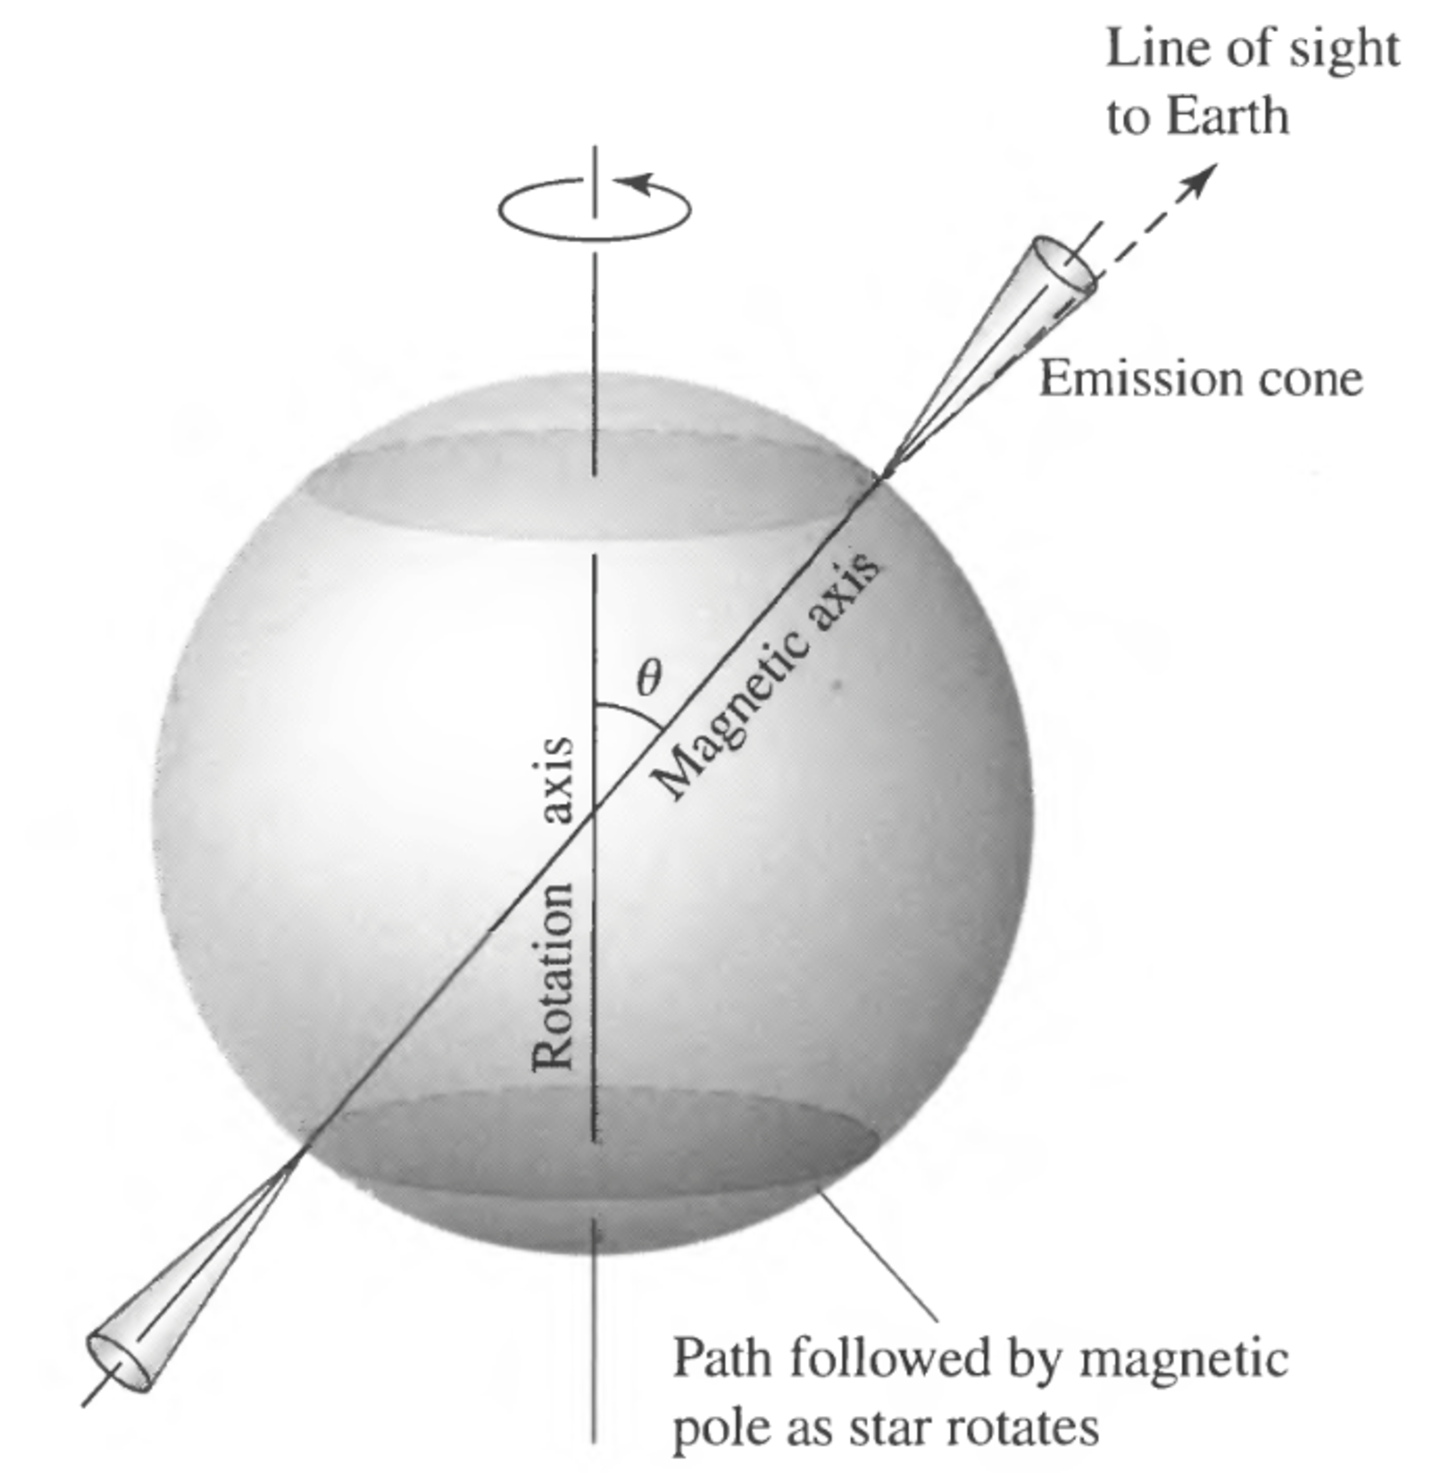
\includegraphics[width=\textwidth]{chapters/introduction/figures/pulsar_model.pdf}
  \end{center}
  \caption{The simplest model of a puslar. This
  figure is taken from \citep{carroll_2006_introduction-modern}.
  }
  \figlabel{pulsar_model}
\end{figure}

The simplest model of a pulsar is that it is a rotating dipole magnet
with the rotation axis and the magnetic axis offset by an angle
$\PulsarRotationAngle$.
A diagram of this model is shown in \figref{pulsar_model}.
The energy output from the pulsar is
then assumed 
to come from rotational kintetic energy stored in
the netutron star which is released as the pulsar
spins down. 

Both the period \period and the period derivative
$\perioddot=d\period/d\time$ can be directly observed for a pulsar.
Except in a few millisecond pulsars which are being sped up
through accreition (see for example \cite{falanga_2005_integral-observations}),
pulsars are slowing down ($\perioddot<0$).

We write the rotational kinetic energy as
\begin{equation}\eqnlabel{rotational_energy}
  \energyrotational = \tfrac{1}{2} I \angularfrequency^2
\end{equation}
where $\angularfrequency = 2\pi/\period$ is
the angular frequency of the pulsar and
\momentofinertia is the moment of inertia.

For a uniform sphere,
\begin{equation}
  \momentofinertia = \frac{2}{5} M R^2
\end{equation}
Assuming a canonical pulsar as was described in \secref{pulsar_pwn_system},
we find a canonical moment of inertia of 
$\momentofinertia=10^{45}\unitspace\gram\unitspace\cm^{-2}$.

We make the conection between the pulsar's spin-down
energy and the rotational kinetic energy as $\energydot = -
\derivative\energyrotational/\dtime$. Using this,
\eqnref{rotational_energy} can be rewritten as
\begin{equation}\eqnlabel{edot_from_rotation}
  \energydot = I \angularfrequency \angularfrequencydot
\end{equation}

It is believed that as the pulsar spins down, the this rotational energy
is released as pulsed electromagnetic radiation and also as a wind of
electrons and positrons accelerated in the magnetic field of the pulsar.

If the pulsar were a pure dipole magnet, its radiation would be
described as \citep{gunn_1969_magnetic-dipole}
\begin{equation}\eqnlabel{edot_pure_dipole}
  \energydot \propto \frac{\MagneticField^2 \PulsarRadius^6 
  \angularfrequency^4 \sin^2\PulsarRotationAngle}{
  \speedoflight^3}
\end{equation}

Combinding equationts \eqnref{edot_from_rotation} and
\eqnref{edot_pure_dipole}, we find that for a pure dipole magnet,
\begin{equation}\eqnlabel{breaking_index_dipole}
\angularfrequencydot \propto \angularfrequency^3.
\end{equation}

In the few situations in which this relationship has been
definitivly measured, this relationship does has not hold.
We generalize \eqnref{breaking_index_dipole} as:
\begin{equation}\eqnlabel{angular_frequency_derivative_relation}
  \angularfrequencydot \propto \angularfrequency^\breakingindex
\end{equation}
where $\breakingindex$ is what we call the pulsar breaking index. 
And we note that \eqnref{angular_frequency_derivative_relation}
we can can solve for \breakingindex by taking the derivative of the equation
\begin{equation}
  \breakingindex = \frac{\angularfrequency \angularfrequencydotdot}{\angularfrequencydot^2}
\end{equation}

The breaking index is hard to measure due to timing noise and glitches
in the pulsar's phase. To this date, it has been meausred in eight 
pulsars (cite \url{http://iopscience.iop.org/2041-8205/741/1/L13/pdf/2041-8205_741_1_L13.pdf}),
and in all situations $\breakingindex<3$. This suggests 
that there are additional processes besides magnetic
dipole radiation that contribute to the energy release
(cite Blandford \& Romani 1988 \url{http://adsabs.harvard.edu/abs/1988MNRAS.234P..57B})

\eqnref{angular_frequency_derivative_relation} is
a Bernoulli differential equation which can be integrated to solve for time:
\begin{equation}\eqnlabel{pulsar_age}
  T = \frac{\period}{(\breakingindex-1) \absval{\perioddot}}
  \left(
  1-\left(\frac{\period_0}{\period}\right)^{(\breakingindex-1)}
  \right)
\end{equation}
For a canonical $\breakingindex=3$ pulsars which is
relativly old $\period_0 \ll \period$, we obtain
what is called the characteristic age of the pulsar:
\begin{equation}
  \pulsarage = \period/2\perioddot.
\end{equation}

Using \eqnref{edot_from_rotation} and \eqnref{breaking_index_dipole}, we can solve
for the spin-down evolution of the pulsar
as a function of time
\citep{pacini_1973_evolution-supernova}
\begin{equation}\eqnlabel{energy_dot_vs_time}
    \energydot(t) = \energydot_0
    \left(
    1 + \frac{\time}{\SpinDownTimescale}
    \right)^{-\frac{(n+1)}{(n-1)}}
\end{equation}
where
\begin{equation}
  \SpinDownTimescale \equiv \frac{\period_0}{(\breakingindex-1)\absval{\perioddot_0}}.
\end{equation}


\eqnref{angular_frequency_derivative_relation}, \eqnref{pulsar_age},
and \eqnref{energy_dot_vs_time} show us that given the current \period,
\perioddot, \energydot, $\period_0$, and breaking index \breakingindex,
we can calculate the pulsar's age and energy-emission history.

In a few situations, the pulsar's age is well known and the breaking index can be
measured, so $\period_0$ can be infered. See \cite{kaspi_2002_constraining-birth}
for a review of the topic. For other sources, attempts have been
made to infer the initial spin-down age based on the dynamics of an
associated \ac{SNR}/\ac{PWN} \citep{van-der-swaluw_2001_inferring-initial}.

\subsection{Pulsar Magnetosphere}

\begin{itemize}
  \item What fraction of pulsar energy is released observationally
\item "While the pulsars emit in the radio band a tiny <= $10^{-6}$
fraction of their rotational energy (Manchester \& Taylor 1977), the
γ-ray luminosities of some of the EGRET pulsars above 100 MeV exceed
one per cent of their spin-down luminosities." -- aharonian\_2003\_exploring-physics
  \item What fraction is released in PWNe?
\item Cite magnetospheric emission model from \cite{gold_1968_rotating-neutron}.
  \item Good discussion in dalton\_2011\_identication-gamma-ray
\end{itemize}

\subsection{Pulsar Wind Nebulae}

The basic picture of 
the physics of \acp{PWN} comes from \cite{rees_1974_origin-magnetic}
and \cite{kennel_1984_magnetohydrodynamic-model}.
A wind of electrons and positrons escape from the pulsar's
magnetosphere and form a bubble pressing into 
the \ac{SNR}. The radius of the bubble (\radiusterminationshock)
is the radius where the ram pressure from the wind
equals thepressure of the gas in the \ac{SNR}.
The ram pressure is computed as the energy in the
bubble $\energydot \radiusterminationshock/c$
divided by the volume $4\pi\radiusterminationshock^3/3$:
\begin{equation}
  \radiusterminationshock = \sqrt{\frac{\energydot}{\tfrac{4}{3}\pi \pressureISM \speedoflight}}.
\end{equation}
Here, \pressureISM is the pressure in the SNR.
Typical values for the termination shock are 0.1\unitspace\parsec
which creats an angular size $\sim$ \acp{arcsec} for distances $\sim\kiloparsec$
\citep{gaensler_2006_evolution-structure}.





\begin{itemize}
\item
"Just after discovery of pulsars, Gunn \& Ostriker (1969) suggested
that par- ticles can be accelerated to very high energies in the pulsar
wind zone." -- "Relativistic Astrophysics and Cosmology" by Shapiro
  \item
    ``Rees \& Gunn (1974) pointed out that pulsar wind terminates in
    a standing reverse shock due to the interaction of a wind with a
    supernova envelope. The details of such model were constracted in a
    steady state, spherically symmetric situation by Kennel \& Coroniti
    (1984a) and in the time de- pendent picture by Emmering \& Chevalier
    (1987). The standing shock deccelerates and heats the e* wind.'' -- 
    ``Relativistic Astrophysics and Cosmology'' by Shapiro
  \item ``Following this discovery, a theoretical understanding was
  soon developed in which the central pulsar generates a magnetized
  particle wind, whose ultrarelativistic electrons and positrons radiate
  synchrotron emission across the electromagnetic spectrum (Pacini \&
  Salvati 1973, Rees \& Gunn 1974). The pulsar has steadily released
  about a third of its total reservoir of ???? ergs
  of rotational energy into its surrounding nebula over the last 950
  years. This is in sharp contrast to shell-like SNRs, in which the
  dominant energy source is the ??? ergs of kinetic energy
  released at the moment of the original SN explosion.''  -- \cite{gaensler_2006_evolution-structure}
  \item 
    What is terminaltion shock of \glspl{PWN}. -- described in Adam Van Etten's thesis
  \item 
    How is pulsar outflow accelerated at shock?
  \item Discuss magnetization stuff :
    \begin{enumerate}
      \item see page 76 in "Relativistic Astrophysics and Cosmology" by Shapiro
    \end{enumerate}
\end{itemize}

\todo[inline]{Discuss pulsar evolution ``The Evolution and Structure of
Pulsar Wind Nebulae'' -- Bryan M. Gaensler and Patrick O. Slane}

\todo[inline]{Describe Mattana's work on \glspl{PWN}: ``On the evolution of
the Gamma- and X-ray luminosities of Pulsar Wind Nebulae''}

"At the termination shock particles are pitch-angle scattered and further
accelerated to ultra-relativistic energies. These energetic particles
radiate across the electromagnetic spectrum in synchrotron and inverse
Compton components from radio to TeV (1 TeV = 1012 electron volts)
energies, resulting in a pulsar wind nebula (PWN, PWNe for plural)." -- etten\_2012\_particle-populations

"As has been discussed, pulsar wind nebulae are prominent sources of
very high energy γ-rays. At these wavelengths, emission is caused
by inverse Compton acceler- ation of seed photons by the relativistic
electrons present in the nebula (see Section 1.3.5). As the electron
energies needed to boost photons to these energies are not as large as
that required for synchrotron emission to occur, inverse Compton emission
is seen at the extremes of the nebula where synchrotron emission can no
longer be observed and as such older pulsar wind nebulae are observed to
be much larger in VHE γ-rays than their X-ray counterparts. In addition
to this, inverse Compton emission is seen in the unshocked wind area of
the PWN as the electrons present are energetic enough to produce inverse
Compton radiation even if they are unable to produce synchroton radiation" -- keogh\_2010\_search-pulsar
